\chapter{Minimum Broadcast Time}\label{sec:mbt}

Broadcasting is the information dissemination process in a communication network.
\textsc{The Minimum Broadcast Time (MBT)} problem is identified by a set of communication devices (nodes), among which some selected ones act as originators of a signal.
The number of originators is at least one, and we refer to them as \emph{sources}.
The task is to spread a signal from the sources to the remaining nodes along pre-defined communication links in a shortest possible time.
In general, communication links are not present between every two nodes.
The continuous time is divided into discrete time steps.
The communication among the nodes must fulfill the following rules:
\begin{enumerate}
\item Each transmission takes place between two adjacent nodes.
\item Each transmission requires one time step.
\item Each node can participate in at most one transmission per time step.
\end{enumerate}

Although this communication protocol is primarily considered as a thoretical model, 
it appears in various practical applications such as communication among computer processors and telephone networks.
Military command, control, communication, computers, intelligence, surveillence and reconnaissance (C4ISR) pose another application for these models \cite{dekker02}.
In satellite networks, even though the communication is wireless, signals have to cover large distances, 
and so the information is sent from one satellite to one of its neighbours at a time.
The MBT problem was studied in the context of an existing Chinese BeiDou Global Navigation Satellite System~\cite{chu17}.

\section{Network Model and Definitions}

The communication network is determined by a graph $G=(V,E)$ and a subset $S\subseteq V$ of sources.

\begin{definition}\label{def:mbt}
The broadcast time $\tau(G,S)$ of $S\subseteq V$ in $G$ is defined as the smallest integer $t\geq 0$
for which there exist a sequence $V_0\subseteq\dots\subseteq V_t$ of node sets and a function $\pi:V\setminus S\mapsto V$, satisfying:
\begin{enumerate}
\item $V_0=S$ and $V_t=V$,
\item for all $v\in V\setminus S, \left\{v,\pi(v)\right\}\in E$,
\item for all $k=1,\dots,t$ and all $v\in V_k$, $\pi(v)\in V_{k-1}$, and
\item for all $u,v\in V_k\setminus V_{k-1}$, $\pi(u)=\pi(v)$ only if $u=v$.
\end{enumerate}
\end{definition}
A node is said to be \emph{informed} at a given time if it is a source, or it already has received the signal from some other node. Otherwise, the node is said to be \emph{uninformed}.
Consequently, the set of informed nodes is initially exactly the set of sources.
Each node set $V_i$, $0\leq i\leq t$ consists of nodes informed in time step $i$.
The function $\pi(u)$ determines a parent node which forwarded the signal to node $u$.
With this interpretation, the conditions 1.-4. of Def.~\ref{def:mbt} can be translated into natural language as 
\begin{enumerate}
\item Initially the only informed nodes are the sources, and at the end of the transmission, all nodes are informed.
\item Nodes send signal along communication links defined by the set of edges.
\item En each time step, a node is informed by its parent who was informed in the previous time step.
\item A node can inform only one child node at a time.
\end{enumerate}

Any feasible solution determines a \emph{communication forest} $\mathcal{F}$ with the set of nodes $V$.
Arcs in $\mathcal{F}$ are induced by the communication: if a node $u$ sends a message to $v$, $(u,v)$ is an arc in $\mathcal{F}$.
It is easily verified that the $\mathcal{F}$ contains arborescences rooted at distinct sources.
Individual arborescences in $\mathcal{F}$ are referred to as \emph{communication trees}.
Let $T_s=\left(V_{T_s},A_{V_s}\right)$ denote the communication tree rooted at source $s\in S$, and define the function $\alpha:V\to S$ such that $v\in V_{T_{\alpha(v)}}$ for all $v\in V$.
That is, $\alpha$ associates a node $v$ with the source at which the communication tree containing $v$ is rooted.
For an arc $(u,v)$ in a given communication tree, the integer $t_{u,v}$ denotes the time step in which node $u$ informs $v$.
%For any communication tree $T_s$, let $T^i_s$ be the subtree of $T_s$ induced by the set of nodes with distance at most $i$ edges from $s$.
%Analogously, let $D^i=\left\{T_s^i: s\in S\right\}$.

Formally, the optimization MBT problem is defined as follows:
\begin{problem}\label{mbt:opt}
Given $G=(V,E)$ and $S\subseteq V$, find $\tau(G,S)$. 
\end{problem}
In the literature, authors often consider the decision version, because some of the theoretical results depend on a given deadline.
\begin{problem}\label{mbt:dec}
Given $G=(V,E)$, $S\subseteq V$,  and a deadline $t\in \mathbb{Z}^+_0$, does $\tau(G,S)\leq t$ hold? 
\end{problem}

Even though the set of sources in a MBT instance is an arbitrary subset of $V$, the following concept assumes a single source.
In a given graph $G$, any node can be a source.
Different sources in $G$ form MBT instances with generally different broadcast times.
The \emph{broadcast center} of a graph is the set of all nodes having the smallest broadcast times, i.e., $\arg\min\left\{\tau(G,\{v\}):v\in V\right\}$.

In $c$-broadcastting, which is a generalization of regular broadcasting, a signal can be sent to up to $c$ nodes adjacent to an informed node in each time step.
%\section{Problem Definition}

%\section{Broadcast Graphs}

\section{Computational Complexity}

MBT has been thoroughly studied from the perspective of computational complexity and approximability, particularly in the early 90'.
Its NP-completeness or belonging to P was proved for various graph classes and values of deadline $t$.

It has been shown that the problem is NP-complete for arbitrary graphs \cite{garey79} and few years later, 
this result was obtained for arbitrary graphs with deadline $t=4$ and a single source by reduction from \textsc{3D Matching}~\cite{slater81}. 
The same work also contains an $\mathcal{O}(n)$ algorithm for the determining broadcast time of a tree with a single source. 
As a by-product, this algorithm determines the broadcast center of the input tree.

These results are improved and extended in~\cite{jansen95}, where the authors exploit the properties of the NP-complete problem \textsc{Planar 3-SAT}.
First, they prove that another satisfiability problem, referred to as \textsc{Planar 3,4-SAT}, is NP-complete, and subsequently use this property to show that MBT is NP-complete for:
\begin{itemize}
\item bipartite planar graphs, deadline $t=2$, and maximum degree at most 3,
\item split graphs with deadline $t=2$,
\item chordal graphs with a single source, 
\item planar graphs with a single source and maximum degree at most 3, 
\item bipartite planar graphs with maximum degree at most 3 and a single source,
\item grid graphs with deadline $t=2$ and maximum degree at most 3,
\item grid graphs with a single source, and
\item complete grid graphs with deadline $t=2$. 
\end{itemize}
The question whether MBT is NP-complete for split graphs with a single source is stated as open.
Another complexity result proving that MBT remains NP-complete for 3-regular planar graphs with constant deadline $t\geq 2$ 
is given in \cite{middendorf93} by reduction from \textsc{Exactly-one-in-three-3-SAT}.

The complexity results above typically exploit sophisticated reductions.
We provide a very simple and straightforward proof of NP-completeness of MBT for deadline at most $t=3$ on bipartite graphs with maximum degree at most 3.
There are many restrictions on SAT that preserve NP-completeness.
We concentrate on the variant of 3-SAT with the property that each variable is restricted to appear at most three times, and each literal at most twice. 
This problem is known as \textsc{3-3-SAT}, and its NP-completeness proof can be found in~\cite{papadimitriou94}. 
Note that in this particular version of 3-SAT, it can no longer be assumed that each clause consists of exactly 3 literals.
Further, the assumption about at most two occurrences of a literal is automatic, 
because a formula $\varphi$ that contains a variable $x$ that appears only as a positive or only as a negative literal 
can trivially be transformed into $\varphi'$ that does not contain $x$ at all, 
such that $\varphi$ is satisfiable if and only if $\varphi'$ is satisfiable.

We now define the association between \textsc{3-3-SAT} and the decision version of MBT (Prob.~\ref{mbt:dec}).
For that purpose, consider the following instance 
\begin{equation}
\varphi=(x_1\vee x_2\vee x_3)\wedge(\bar{x}_1\vee x_4)\wedge(x_2\vee \bar{x}_3 \vee\bar{x}_4)\wedge(\bar{x}_1\vee \bar{x}_3)\wedge \bar{x}_2 
\label{eq:phi}
\end{equation}
of \textsc{3-3-SAT} with variables $x_1,\dots, x_n$ and clauses $c_1,\dots,c_m$, reducing to the instance of Prob.~\ref{mbt:dec} in Fig.~\ref{fig:mbtnpc}.
\begin{figure}
\centering
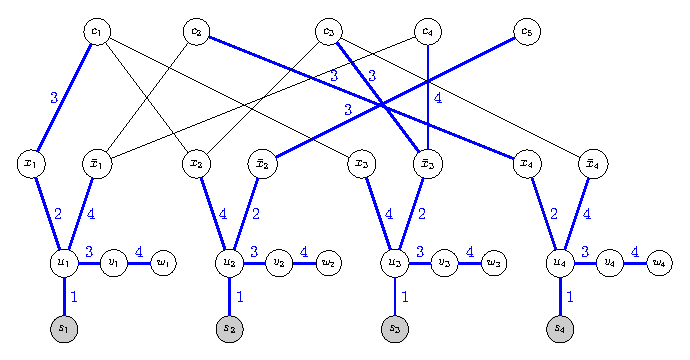
\includegraphics{figurer/mbtnpc.eps}
\caption{Reduction from formula $\varphi$ (Eq.~\eqref{eq:phi}) of \textsc{3-3-SAT} to an instance of MBT with deadline 3 and maximum node degree 3}
\label{fig:mbtnpc}
\end{figure}
For each variable $x_i$, we construct a gadget comprising five $x_i$, $\bar{x}_i$, $u_i$, $v_i$, $w_i$, where $u_i$ is a source, $i=1,\dots n$ .
The first two nodes represent possible literals associated with the variable $x_i$.
The gadget further contains four edges, $\{u_i,x_i\}$, $\{u_i,\bar{x}_i\}$, $\{u_i,v_i\}$, and $\{v_i,w_i\}$.
For each clause $c_j$, there is a node $c_j$ and whenever the clause $c_j$ contains a literal $x_i$ ($\bar{x}_i$), there is an edge $\{c,x_i\}$ ($\{c,\bar{x}_i\}$).
%We therefore have clause nodes of degree at most 3, because $\varphi$ is in 3-CNF.
%Nodes representing literals are connected to at most two clause nodes, which is implied by the restriction imposed on $\varphi$.

\begin{proposition}\label{lemma:mbtred}
MBT is NP-hard.
\end{proposition}
\begin{proof}\label{prop:mbtnpc}
Let $\varphi$ be satisfiable.
A source node $u_i$ sends the signal towards the node representing the literal that is evaluated as true in the given truth assignment.
In the next two time steps, the signal is further relayed to the nodes representing clause that are satisfied by the literal.
As each literal can cause satisfaction of up to two clauses, the corresponding clause nodes receive the signal from the respective literals within the deadline 3.
Nodes $u_i$ must receive the signal in the time step 2, in order to reach $w_i$ on time.
Thus, the node representing the literal evaluated as false receives the signal in time step 3.

Conversely, let the constructed instance of MBT have broadcast time no more than 3.
In a solution $T$ to the instance (highlighted as blue in Fig.~\ref{fig:mbtnpc})  $\arg\min_{v\in\{x,\bar{x}\}}\{t_{u_x,v}\}$ represents the assignment of truth value to the variable $x$.
The presence of an arc entering a clause node $c$ in $T$ indicates that a truth value of certain variable caused satisfaction of clause $c$.
%The truth evaluation of clauses can be retrieved by looking up nodes representing literals that receive the signal in time step 1.
The auxiliary path $(u_x,v_x,w_x)$ ensures that the clause satisfaction is modeled correctly.
As $t_{u_x,v_x}\leq 2$, one of $t_{u_x,x}$ and $t_{u_x,\bar{x}}$ must be 3, 
and thereby the arc that would incorrectly indicate satisfaction of a clause that is not satisfied by the selected truth assignment would have cost 4, which is not allowed.
It is possible to have an arc outgoing from a clause node of cost 3, but the second endpoint is always a node representing some literal $y$, but the arc $(u_y,y)$ is already a part of $T$.

The correctness of the truth valuation is ensured by the existence of nodes $v_i$, so that the node representing literal that is evaluated as false is informed in time step 3, 
and thereby cannot forward the signal to any clause nodes.
\end{proof}

\begin{proposition}
The decision version of MBT (Prob.~\ref{mbt:dec} is NP-complete for bipartite graphs with maximum node degree 3 and deadline 3.
\end{proposition}
\begin{proof}
In \cite{slater81}, a polynomial algorithm for MBT in trees is devised.
As the sequence of vertices $V_0\subseteq\dots\subseteq V_t$ and function $\pi$ in Def.~\ref{def:mbt} determine a unique forest $\mathcal{F}$ of arborescences,
it can be verified in polynomial time whether the broadcast time of each braodcast tree in $\mathcal{F}$ does not exceed 3, proving that MBT belongs to NP.
This concludes together with Lemma~\ref{lemma:mbtred} that MBT is NP-complete for deadline at most 3.

As each literal appears at most twice in $\varphi$, the degree of nodes representing literals is at most 3. 
Each clause node has degree at most 3 since $\varphi$ is in 3-CNF.
Degrees of nodes $u_i$, $v_i$, and $w_i$ do not depend on $\varphi$, and have degrees 3, 2, and 1, respectively.
Thus, none of the node degrees in the constructed MBT instance exceeds 3.

Nodes of the constructed graph are divided into two disjoint sets $X=\{u_i,w_i,c_j\}$, $i=1,\dots,n$, $j=1,\dots,m$ and $Y=\{x_i,\bar{x}_i,v_i\}$, $i=1,\dots,n$.
The graph is bipartite as there are no edges between any two nodes within $X$ or $Y$.
\end{proof}

\section{Integer Linear Programming Models}

A straightforward ILP formulation of MBT has been proposed in Paper IV together with a suitable solution method.
Independently, a similar formulation has recently been published in \cite{desousa18}.
In the following, we present an unpublished ILP model for MBT.

\subsection{Binomial Tree Model}

A \emph{binomial tree} $B^k$ of order $k$ is an ordered tree defined recursively as follows \cite{cormen01}:
\begin{itemize}
\item The binomial tree $B^0$ consists of a single node.
\item The binomial tree $B^k$ has a root with $k$ children where the $i$-th child is the root of a binomial tree of order $k-i$, $i=1,\dots,k$.
\end{itemize}
An example of $B^3$ is depicted in Fig.~\ref{fig:beta}.
%If a solution to MBT consists of broadcast trees that are binomial, the number of informed nodes doubles in each time step.
For a given time step $k$, the maximum number of informed nodes within $k$ steps is $|S|2^k$.
This occurs when the solution of MBT consists of broadcast trees that are binomial.
%Any broadcast tree can be regarded as pruned binomial tree.
%Problem \ref{prob:min} can therefore be restated as finding a partition of $G$ into $m$ pruned binomial trees
\begin{observation}
\label{obs:btspread}
If $r$ is the root of $B^k$, then $\tau(B^k,\{r\})=k$.
\end{observation}
\begin{figure}
\centering
	
\includegraphics{figurer/btindex.eps}
\caption{A binomial tree with nodes labeled by their positions}
\label{fig:beta}
\end{figure}

Let $k\in \mathbb{N}$ and $I=\{1,\dots,2^k\}$.
A directed binomial tree $B^k=(V_{B^k},A_{B^k})$ with arcs oriented towards the leaves has a regular structure that allows to define a systematic numbering of nodes so that a node number determines unambiguously a \emph{position} in $B^k$.
That is, we need an applicable bijective function $\beta:V_{B^k}\to I$.
A suitable bijection $\beta$ assigns values from $I$ to nodes increasingly with decreasing outgoing degree.
In case of a tie, $\beta$ takes the smaller value at the node whose parent node is assigned the smaller value.
%If there is an ambiguity, a node whose parent has a lower number is assigned a lower number.
This function is defined recursively as
\begin{equation*}
\label{eq:beta}
\beta(v)=\begin{cases}
1,\text{ if } v \text{ is the root of } B^k,\\
\beta(u) + 2^{k-deg^+(v)-1}, \text{ if } \pi(v)=u.%(u,v)\in A_{B^k},\text{ otherwise}.
\end{cases}
\end{equation*}
Nodes in Fig. \ref{fig:beta} are labeled with their positions according to $\beta$.
\begin{definition}
For a node $v\in V'$ with position $i=\beta(v)$, define the corresponding \emph{chidl position set}, $C(i)$, 
consisting of positions of child nodes of $v$ in $B^k$.
That is,
$$
	C(i)=\left\{\beta(u): \pi(u)=v,\text{ i.e., } u \text{ is a child of } v \text{ in } B^k\right\}.
$$
\end{definition}
By the definition of $\beta$, it follows that 
\begin{equation}
\label{eq:c1}
C(i)=\{2^j+i:j=\lceil\log_2 i\rceil,\dots,k-1\}.
\end{equation}

The idea behind this model is that every broadcasting from a single source follows arcs of a (potentially pruned) binomial tree.
The value of $\tau(G,S)$ can be retrievd from the maximum among the positions assigned to nodes.
Intuitively, an advantage of this concept is when applied on dense graph instances where feasible solutions should be found quickly.
To see this, consider a complete graph $K_n$.
Any assignment of positions $1,2,\dots,n$ to nodes is valid and optimal. 
Moreover, a broadcast time of dense graphs is often equal to the lower logarithmic bound.
Near complete graphs have therefore many optimal solutions, which are expected to be discovered easily.
%\begin{problem}
%\label{prob:dec}
%Given $G=(V,E)$, $S\subseteq V$ and $t\in \mathbb{N}$, is there a sequence $S=V_0\subseteq\dots\subseteq V_t=V$
%and a mapping $\pi:V\setminus S\to V$, such that for each $v\in V\setminus S:\{v,\pi(v)\}\in E$ and for each  $u,v\in V_i\setminus V_{i-1}: \pi(u)\neq \pi(v)\Leftrightarrow u\neq v$?
%\end{problem}
%For a delay $t$, at most $s\cdot 2^t$ nodes can be informed within $t$ steps.
%Therefore, we assume $n\leq 2^ks.
%This can be achieved when the broadcast forest $T$ consists of binomial trees $B^t$ of order $t$ rooted at sources $s\in S$.
%Hence, if there is a partition of $G$ into $s$ pruned binomial trees of order at most $t$ rooted at sources, then $(G,S,t)$ is a YES instance of Problem \ref{prob:dec}.
%Finding a partition of $G$ into $s$ pruned binomial trees can be equivalently formulated as finding a partition of $G''$ into $s$ (complete) binomial trees,
%where $G''$ is constructed from $G$ as follows:
%Let $\alpha\coloneqq s\cdot 2^k-|V|$, and let $K_\alpha=(V_\alpha,E_\alpha)$ be a complete graph on $\alpha$ nodes.
%Each node in $K_\alpha$ is connected to every node $v\in V$ in the original graph $G$.
%Thus, $G''=(V'',E'')$ with $V''=V\cup V_\alpha$ and $E''=E\cup E_\alpha\cup \{\{u,v\}: u\in V \wedge v\in V_\alpha\}$.
%The set of arcs $A''$ is constructed by creating two arcs of opposite orientation for each edge, but arcs with orientation from $V_\alpha$ to $V$ are excluded.
%Formally, $A''=A\cup\{(u,v),(v,u): \{u,v\}\in E_\alpha\}\cup\{(u,v):u\in V \wedge v\in V_\alpha\}$.

%\begin{observation}\label{obs:deg}
%For each $i\in\{1,\dots,t\}$, the set $\{v\in V^t: 1\leq\beta(v)\leq2^i\}\setminus\{v\in V^t:1\leq\beta(v)\leq2^{i-1}\}$ contains nodes with out-degree $t-i$.
%\end{observation}
%\begin{observation}\label{obs:childdeg}
%Children of $v\in V^t$ with $\text{deg}^+(v)=\ell$ have out-degree $0,\dots,\ell-1$.
%\end{observation}
\subsubsection{The formulation}
Consider a graph $G'=(V',E')$ constructed  by adding an auxiliary universal node $v_0$ to $G$.
The set of nodes and edges is then $V'=V\cup \{v_0\}$ and $E'=E\cup\{\{v_0,v\}:v\in V\}$.
So far we have considered binomial trees $B^k$ of an arbitrary order $k$.
For finding a valid assignment of positions to the nodes, we need a binomial tree of order at least $\tau(G,S)$.
As $\tau(G,S)$ is unknown, we must determine some suitable upper bound $\bar{t}$ on $\tau(G,S)$.  
\begin{observation}
A trivial upper bound on $\tau(G,S)$ is $n-|S|$.
\end{observation}
The ILP formulation based on a partition into binomial trees uses variables
$$
z_{j}=
\begin{cases}
1, \text{ if } j\leq \bar{t},\\
0, \text{ otherwise},
\end{cases}
y_{is}^v=
\begin{cases}
1, \text{ if } \beta(v)=i \text{ and } \alpha(v)=s,\\
0, \text{ otherwise},\\
\end{cases}
$$
where $v\in V'$, $i\in I=\left\{1,\dots,2^{\bar{t}}\right\}$, $s\in S$ and $0\leq j\leq \bar{t}$.
With the definition of $G'$ above, it is straightforward to specify constraints that enforce desired values for $y$-variables.
Whenever $y_{is}^{v_0}=1$, it indicates that the binomial tree rooted at $s$ is pruned at node with position $i$.
%An obvious weakness of this approach is  that the number of nodes increases to $|V''|=\mathcal{O}(ns)$, and the dimension of variables is thus $\mathcal{O}(n^2s^2)$.
%However, once a suitable partition is found, the arcs of binomial trees contained in $K_\alpha$ can be diversely shuffled while preserving the layour of binomial trees in $G$.
%Instead of adding the entire complete graph $K_\alpha$, a single node $v_0$ with a loop $(v_0,v_0)$ is connected as an apex to the original $G$.
%Let us denote this multigraph as $G'=(V',E')$, where $V'=V\cup\{v_0\}$, $E'=E\cup\{\{u,v_0\}:u\in V\}\cup\{\{v_0\}\}$.
%The arc set is then analogously defined as $A'=A\cup\{(u,v_0): u\in V\}\cup\{(v_0,v_0)\}$.
%The requirement for partition into binomial trees has to be adjusted accordingly.
%The subtrees contained in $G$ remain unchanged, every arc $(u,v)\in A^k_i, i=1,\dots,s$ in $G''$ with $u\in V$ and $v\in V_\alpha$ becomes $(u,v_0)$ in $G'$,
%and every $(u,v)\in A_\alpha$ becomes $(v_0,v_0)$.
%So, $v_0$ acts as a universal node that can substitute several nodes in each binomial tree.
The formulation based on binomial trees is the following:
\begin{subequations}\label{mod:partition}
\begin{align}
\notag &\min\sum\limits_{j=0}^{\bar{t}}z_j,\\
\notag \text{s. t. } \\
\label{mod:part:nodeBelongs} \sum\limits_{i\in I}\sum\limits_{s\in S}y^v_{is} & = 1 & v\in V,\\
\label{mod:part:treeHasIJ} \sum\limits_{v\in V'}y^v_{is} & = 1 & i\in I,s\in S,\\
\label{mod:part:source1} y_{1s}^s & = 1  & s\in S,\\
%\label{mod:part:noReturn} y^u_{ij}+y^v_{lj} &\leq 1 & i\in I,l\in C(i), j\in J, u\in V_\alpha,v\in V,\\
%\label{mod:part:followArcs} y^u_{is}+y^v_{\ell s} &\leq 1 & i\in I,\ell\in C(i), s\in S, u,v\in V',(u,v)\not\in A',\\
%\label{mod:part:followArcsA} y^u_{is}+y^v_{\ell s} &\leq 1 & i\in I,\ell\in C(i), s\in S, u,v\in V,\{u,v\}\not\in E,\\
%\label{mod:part:followArcsB} y^{v_0}_{is}+y^v_{\ell s} &\leq 1 & i\in I,\ell\in C(i), s\in S, v\in V,\\
\label{mod:part:followArcsA}y^{v_0}_{is}+y^u_{i s} + \sum\limits_{v\in V\setminus N(u)}y^v_{\ell s}&\leq 1 & u\in V,i\in I,\ell\in C(i), s\in S,  \\
\label{mod:part:followArcsB}y^{v_0}_{is}+y^u_{\ell s} + \sum\limits_{v\in V\setminus N(u)}y^v_{i s}&\leq 1 & u\in V,i\in I,\ell\in C(i), s\in S,\\
%\label{mod:part:followArcsA}\sum\limits_{v\in \bar{N}(u)}y^v_{\ell s}&\leq \sum\limits_{v\in N(\bar{N}(u))}y_{is}^{v} & u\in V,i\in I,\ell\in C(i), s\in S,  \\
%\label{mod:part:followArcsB}\sum\limits_{v\in \bar{N}(\bar{N}(u))}y^v_{\ell s}&\leq \sum\limits_{v\in N(u)} y_{is}^{v} & u\in V,i\in I,\ell\in C(i), s\in S,\\
\label{mod:part:yzrel}\sum\limits_{v\in V}y^v_{is} & \leq z_{\lceil\log i\rceil} & i\in I,s\in S,\\
\label{mod:part:dim}y \in \{0,1\}^{I\times S\times V'}, z&\in \{0,1\}^{\bar{t}}.
\end{align}~
\end{subequations}

%As the model represents the decision problem, it suffices to find any feasible solution, and no objective function is needed.
The interpretation of constraints \eqref{mod:part:nodeBelongs} is that every node in the original graph $G$ belongs to exactly one binomial tree.
Note that these constraints are quantified only over $V$ and not over $V'$.
In this way it is achieved that $v_0$ can be regarded as a part of several binomial trees.
By \eqref{mod:part:treeHasIJ} is enforced that exactly one node, possibly $v_0$, is allocated to position $i$ of each binomial tree.
By the summation over $V'$ is ensured, that pruned nodes are collectively represented by $v_0$.
Next, \eqref{mod:part:source1} enforce that source nodes are always the first nodes in corresponding binomial trees, 
in accordance with definition \eqref{eq:beta} of the function $\beta$.
Constraints \eqref{mod:part:followArcsA} and \eqref{mod:part:followArcsB} guarantee that the arcs of binomial trees follow edges in $E$.
In particular, it is enforced by \eqref{mod:part:followArcsA} that if $u$ and $v$ are not adjacent in $G$, 
then $v$ must not have a position of child of $u$ in any binomial tree.
Similarly by \eqref{mod:part:followArcsB}, if $u$ and $v$ are not adjacent in $G$, then $v$ must not act as a parent of $u$ in any binomial tree.
Without \eqref{mod:part:followArcsA} and \eqref{mod:part:followArcsB}, it could be possible to find a feasible solution, 
even when no partition of $G$ into pruned binomial trees exists.
Finally, the relation \eqref{mod:part:yzrel} between $y$ and $z$ variables follows from Obs. \ref{obs:btspread}.
It says that whenever there is a node in a position $i$, then the delay is at least $\lceil\log i\rceil$.

Consider a subset $U\subseteq V$.
Let $N(U)=\left\{v:\left\{u,v\right\}\in E, u\in U\right\}$, and $\bar{N}(U)=V\setminus N(U)$.
Constraints \eqref{mod:part:followArcsA} - \eqref{mod:part:followArcsB} can then be replaced by stronger
\begin{subequations}\label{mod:partition:imp}
\begin{align}
\label{mod:part:imp:followArcsA}\sum\limits_{v\in \bar{N}(u)}y^v_{\ell s}&\leq \sum\limits_{v\in N(\bar{N}(u))}y_{is}^{v} & u\in V,i\in I,\ell\in C(i), s\in S,  \\
\label{mod:part:imp:followArcsB}\sum\limits_{v\in \bar{N}(\bar{N}(u))}y^v_{\ell s}&\leq \sum\limits_{v\in N(u)} y_{is}^{v} & u\in V,i\in I,\ell\in C(i), s\in S.
\end{align}~
\end{subequations}
It is enforced by \eqref{mod:part:imp:followArcsA} that if there is some  non-neighbor $v$ of $u$  with a position $\ell$ in a binomial tree rooted at $s$,
then there must be a neighbor of some non-neighbor of $u$ with position $i$ in the same binomial tree.
Similarly, Constraints \eqref{mod:part:imp:followArcsB} state 
that if there is a node $v$ with position $\ell$ in a binomial tree rooted at $s$ in the complement of neighborhood of all non-neighbors of $u$,
This reflects the obvious fact that if a tree is pruned at some node, all its descendants must also be excluded from the tree.
\subsubsection{Valid inequalities}
Let $W$ be a maximal independent set in $G$.
Model \eqref{mod:partition} is strengthened by
\begin{align}
\label{mod:part:vibasic}
y^{v_0}_{is}+ \sum\limits_{v\in W}(y^v_{is}+y^v_{\ell s})&\leq 1 & i\in I,\ell\in C(i), s\in S,
\end{align}
which exploits the fact that no pair of nodes in $W$ is adjacent, and so there must be no two nodes with adjacent $\beta$-positions.

We now generalize this idea by using the notion of graph power $G^m=(V,E^m)$ commonly defined as a graph with the same set of nodes as $G$,
and an edge between two nodes in $G^m$ is present iff there is a path of length at most $m$ between them in $G$.
For our purposes, we use a slightly modified definition of the edge set
$$E^m=\{\{u,v\}:\text{there exists a path between $u$ and $v$ in $G$ of length $m$}\}.$$
Definition \eqref{eq:c1} can be generalized to descendants of an arbitrary distance $m=1,2,\dots$ from $v$ in $B^k$:
\begin{align}
\begin{split}
	C^{1}(i)&=C(i),\\
	C^{m+1}(i)&=\bigcup_{j\in C^1(i)}C^m(j).
\end{split}
\end{align}
%For a given $m$, let $W_m$ be a maximal independent set in $G^m$.
Further strengthening of model \eqref{mod:partition} is achieved by introducing valid inequalities
\begin{align}
\label{mod:part:vigeneral}
y^{v_0}_{is}+ \sum\limits_{v\in W_m}(y^v_{is}+y^v_{\ell s})&\leq 1 & i\in I,\ell\in C^m(i), s\in S,1\leq m\leq \Delta_G-1.
\end{align}
Clearly, inequality \eqref{mod:part:vibasic} is included in \eqref{mod:part:vigeneral} for $m=1$.
The distance between positions $i$ and $\ell=C^m(i)$ in a binomial tree is $m$.
The maximal independent set $W_m$ contains nodes such that length of any path between any two nodes is different from $m$,
and so there cannot be two nodes in $W_m$ with positions $i$ and $\ell$ at the same time.

\subsubsection{Symmetry removal}
Another improvement of this model is achieved by a symmetry removal.
If a broadcast tree is identical to a binomial tree, we notice that nodes with positions from $C(i)$, i.e., children of some node $v$ with $\beta(v)=i$, are informed in increasing time steps.
For example in $B^3$, $C(2)=\{4,6\}$ and the corresponding nodes are informed in time step 2 and 3, respectively.
If a position $\ell\in C(i)$ corresponds to a node of a binomial tree that is pruned (if $y^{v_0}_{\ell s}=1$ for some $s\in S$),
all positions $j\in C(i)$ such that $j>\ell$ can also be pruned.
Thus, adding
\begin{align}
\label{mod:part:sr}
y^{v_0}_{js}&\leq y^{v_0}_{\ell s}&i\in I,j,\ell\in C(i),j<\ell, s\in S
\end{align}
to the model reduces the set of feasible solutions, while preserving at least one optimal solution.

\subsubsection{Decision version}\label{sec:mbt:ilp:dec}

To determine whether a given deadline $k$ is sufficient for broadcasting in an instance $(G,S)$ of MBT, consider the following ILP model:
\begin{subequations}\label{mod:genmatch}
\begin{align}
\notag \max\sum\limits_{v\in V}&\sum\limits_{i\in I}\sum\limits_{s\in S}   y_{is}^v,\\
\notag \text{s. t. } \\
\label{mod:genmatch:nodeBelongs} \sum\limits_{i\in I}\sum\limits_{s\in S}y^v_{is} & \leq 1 & v\in V,\\
\notag\eqref{mod:part:treeHasIJ} - \eqref{mod:part:followArcsB},\\
\label{mod:genmatch:dim}&&y \in \{0,1\}^{I\times S\times V'}.
\end{align}~
\end{subequations}
This model is a modification of formulation \eqref{mod:partition}, and uses the same type of variables.
The objective function is to maximize the number of nodes that are assigned a position in binomial trees.
%In order to determine the minimum broadcast time, 
%we are looking for the minimum $k$ such that each node can be assigned a position from the set $I=\{1,\dots,2^k\}$ while satisfying given constraints.
%The index set $I=\{1,\dots,2^k\}$ depends on the input parameter $k$.
The constraints \eqref{mod:genmatch:nodeBelongs} state that each node belongs to at most one binomial tree.
In contrast to \eqref{mod:part:nodeBelongs}, \eqref{mod:genmatch:nodeBelongs} is an inequality, 
because the binomial trees do not necessarily form a partition of $G$, and so not all nodes have to be used.
The remaining constraints are taken from formulation \eqref{mod:partition}.

The parameter $k$ affects $I$.
If the objective function attains the target value $|V|$, 
it is obvious that positions $\left\{1,2,\dots,2^k\right\}$ can be assigned to all nodes in $G$ under the given constraints, and therefore $\tau(G,S)\leq k$.
If the objective function value is less than $|V|$, then clearly $\tau(G,S)>k$.

An optimal solution to Prob.~\ref{mbt:opt} can be determined by a sequential solving of model \eqref{mod:genmatch} for varying deadlines $k$.
Assume we are given a lower bound $\underline{t}$ and an upper bound $\bar{t}$ on the minimum broadcast time.
Initially, we define the set $I=\{1,\dots,2^{\underline{t}}\}$ and iteratively solve the model while doubling the set $I$ until the objective function attains the value $n$.
That indicates that it is the first iteration in which all nodes are assigned a position, and it can be concluded that the minimum broadcast time is $\log_2|I|=\underline{t}$.
If the target value $|V|$ is not met for $k=\bar{t}-1$, the last iteration with $k=\bar{t}$ does not have to be conducted, as it is already obvious that $\tau(G,S)=\bar{t}$.

It is suggested that the sequence of models is solved for an increasing $k$. 
Different strategies are also available. 
For example, a binary search may seem a more natural way, however, running the model for larger values of $k$ takes significantly more time than for smaller values of $k$.
Furthermore, large graphs tend to have their broadcast time closer to the lower bounds.

\subsubsection{Discussion}

Preliminary experimental results indicate that using binomial tree model for obtaining optimal solutions of MBT instances 
takes longer time copared to the model presented in Paper IV in virtually all tested instances. 
Tab.~\ref{tab:xvsy} shows solution times for two instance sets with number of nodes 50 and 100.
Each instance set is further divided by the number of sources, in this case 1 and 2.
Last parameter that identifies an instance is the number of edges (1st and 6th column).
Each instance is then tested on 
An instance is identified by values $|V|$, $|S|$ and $|E|$.
Each instance is solved by an iterative algorithm described in section \ref{sec:mbt:ilp:dec} on model \eqref{mod:genmatch}
(columns with heading $Y$), and an analogous algorithm on model introduced in Paper IV (columns with heading $X$).

Even this small sample of test instances suggests that the model in Paper IV finds an optimal solution substantialy faster than \eqref{mod:genmatch}.
However, there is a potential in improving the model by means of techniques such as further symmetry removal
and additional valid inequalities following from the concept of unique numbering of nodes in a binomial tree.
Also, it can be seen tha the more sources, the shorter time the computation takes, which is more aparent for model \eqref{mod:genmatch}.
\begin{table}[h]
\begin{centering}
\begin{tabular}{rrrrrrrrrrr}
\multicolumn{5}{c}{$|V|$=50}                                      &~~  & \multicolumn{5}{c}{$|V|$=100}                                     \\\hline
      & \multicolumn{2}{c}{$|S|$=1} & \multicolumn{2}{c}{$|S|$=2} &~~  &       & \multicolumn{2}{c}{$|S|$=1} & \multicolumn{2}{c}{$|S|$=2} \\\hline
$|E|$ & $X$          & $Y$          & $X$          & $Y$          &~~  & $|E|$ & $X$         & $Y$           & $X$         & $Y$           \\\hline
276   & 0.22         & 7.39         & 0.18         & 4.37         &~~  & 1041  & 0.99        & 261.71        & 0.7         & 109.32        \\
262   & 0.19         & 4.76         & 0.2          & 2.67         &~~  & 1078  & 0.78        & 243.66        & 0.84        & 84.45         \\
269   & 0.2          & 8.43         & 0.1          & 2.62         &~~  & 1013  & 1.26        & 326.66        & 0.78        & 141.28        \\
194   & 0.3          & 9.81         & 0.13         & 3.08         &~~  & 798   & 0.74        & 441.31        & 0.39        & 47.28         \\
192   & 0.14         & 2.72         & 0.15         & 3.16         &~~  & 781   & 0.91        & 254.67        & 0.52        & 53.74         \\
188   & 0.16         & 4.75         & 0.09         & 2.26         &~~  & 726   & 0.87        & 299.97        & 0.78        & 225.19        \\
63    & 0.19         & 8.49         & 0.17         & 11.82        &~~  & 125   & 0.57        & 904.51        & 0.54        & 705.06        \\
100   & 0.16         & 7.49         & 0.08         & 2.59         &~~  & 200   & 1.23        & 1126.11       & 0.76        & 298.8        
\end{tabular}
\caption{Comparison of solution time of methods based on model~\eqref{mod:genmatch} and an analogous model in Paper IV.}
\label{tab:xvsy}
\end{centering}
\end{table}

%\section{Inexact Algorithms}

%A number of heuristics methods as well as approximation algorithms along with associated theoretical results have been developed.

\section{Related Problems}

There many communcation protocols for broadcasting in different practical applicatons, leading to  and their description is out of the scope of this thesis.
We therefore describe only the problems closely related to MBT.

\subsection{Broadcast Graphs}

A related problem to MBT is the problem of finding minimum broadcast graphs.
In this settings, broadcast protocol according to Def.~\ref{def:mbt} and  $|S|=1$ are assumed.
A \emph{broadcast graph} is a communication network on $n$ nodes with optimal broadcast time $\lceil \log n\rceil$ regardless of the source.
Every complete graph $K_n$ satisfies this property, yet $K_n$ is not minimal. 
The minimum number of edges in any broadcast graph on $n$ nodes is denoted as $B(n)$.
A \emph{Minimum broadcast graph} is a broadcast graph with $B(n)$.

NP-completeness follows from the same result for MBT.
A long list of paper deals with determining minimum broadcast graph for different number of nodes.
The initial work \cite{farley79} shows minimum broadcast graphs for $n=2^k$ and $n\leq 15$.
Further investigation \cite{harutyunyan99} leads to a technique for constructing broadcast graphs for many values of $n$.

In the generalized $c$-broadcasting, a \emph{$c$-broadcast graph} has a broadcast time $\lceil \log_{c+1} n\rceil$, and analogously, 
$B_c(n)$ denotes the minimum number of edges in any $c$-broadcast graph.
A $c$-broadcast graph with $B_c(n)$ edges is said to be a \emph{minimum $c$-broadcast graph}.
A time-relaxed $c$-broadcasting \cite{mcgarvey16} allows additional $t$ time steps are allowed.
Thus, a time-relaxed $c$-broadcast graph has broadcast time $\lceil \log_{c+1} n\rceil+t$.

Another generalization is the $k$-fault tolerant broadcast problem \cite{liestman85}.
The task is to identify sparse graphs with reliable transmission schemes.
The protocols of a $k$-fault tolerant broadcast graph are predefined in such a way that if any $k$ edges in the protocol fail, the signal still reaches all nodes in the graph.

ILP formulations to construct $c$-broadcast graphs, $k$-fault tolerant $c$-broadcast graphs and minimuim $c$-broadcast graphs are presented in \cite{mcgarvey16}.

\subsection{The Gossiping Problem}

The last poblem mentioned in this overview is \textsc{The Gossiping Problem}, also known as \emph{Total information exchange}.
In this problem, each node is initially given a different message that needs to be distrubuted to all other nodes \cite{chrobak00}.
For this, in each time step the nodes send each other messages consisting of an arbitrary number of pieces of information. 
The standard restriction is that in one time step, a node can communicate with only one of its neighbors. 
One distinguishes 1-way (or half-duplex) mode, where thep information can be sent through a link in only one direction in a single time step, 
and 2-way (or full-duplex) mode, where two nodes may exchange all their information through a link that connects them within a single time step. 
The most intensively studied efficiency criterion in this theory is the number of time steps needed for disseminating all pieces of information to every node \cite{dietzfelbinger04}.
